\documentclass[12pt,a4paper]{article}
\usepackage[utf8]{inputenc}
\usepackage[spanish,es-tabla]{babel}
\usepackage{amsmath}
\usepackage{amsfonts}
\usepackage{amssymb}
\usepackage{graphicx}
\usepackage{float}
\usepackage{hyperref}
\usepackage{booktabs}
\usepackage{caption}
\usepackage{geometry}
\usepackage{xcolor}
\usepackage{titlesec}
\usepackage{array}
\usepackage{enumitem}
\usepackage{subcaption}
\usepackage{listings}
\usepackage{courier}

\geometry{margin=2.5cm}

% Ruta base para las figuras (relativa desde donde se compila el .tex)
% Si compilas desde la carpeta Reporte/, las figuras estan en ../output/figures/
\graphicspath{{../}{../output/figures/}}

\definecolor{themeColor}{RGB}{0,100,60}
\definecolor{themeDark}{RGB}{20,50,40}

\hypersetup{
    colorlinks=true,
    linkcolor=themeColor,
    filecolor=magenta,
    urlcolor=cyan,
}

\titleformat{\section}{\large\bfseries\color{themeColor}}{\thesection}{1em}{}
\titleformat{\subsection}{\normalsize\bfseries}{\thesubsection}{1em}{}

\lstset{
    basicstyle=\ttfamily\small,
    breaklines=true,
    frame=single,
    language=Python,
    showstringspaces=false,
    captionpos=b,
    keywordstyle=\color{themeColor},
    commentstyle=\itshape
}

% ============================================================
% PORTADA
% ============================================================
\begin{document}

\begin{titlepage}
    \centering
    \vspace*{2cm}
    
    {\LARGE\bfseries\color{themeColor} Universidad Autónoma de Querétaro\par}
    \vspace{0.5cm}
    {\large Facultad de Informática\par}
    \vspace{1.5cm}
    
    \rule{\textwidth}{1.5pt}\par
    \vspace{0.5cm}
    {\huge\bfseries Predicción del Precio de Acciones\par}
    {\huge\bfseries de Starbucks (SBUX) mediante\par}
    {\huge\bfseries Random Forest\par}
    \vspace{0.3cm}
    \rule{\textwidth}{1.5pt}\par
    \vspace{1.5cm}
    
    {\large\textbf{Materia:} Aprendizaje Automático\par}
    \vspace{0.5cm}
    {\large\textbf{Profesor:} Dr. Marco Antonio Aceves\par}
    \vspace{0.5cm}
    {\large\textbf{Alumno:} Yhael Salvador Pérez Balderas\par}
    \vspace{1.5cm}
    
    \vfill
    {\large Mayo 2026\par}
\end{titlepage}

% ============================================================
% RESUMEN
% ============================================================
\begin{abstract}
En este trabajo se implement\'o un modelo de \textit{Random Forest} para predecir el retorno logar\'{\i}tmico (\textit{log\_return}) de las acciones de Starbucks (SBUX). Se utilizaron 250 registros diarios del per\'{\i}odo febrero 2025 a enero 2026, con caracter\'{\i}sticas derivadas de precio y volumen (rango diario, volatilidad, volumen transformado, rezagos y variables temporales). El mejor modelo, optimizado mediante validaci\'on temporal, alcanz\'o un $R^{2}$ de 0.028 y un RMSE de 0.0171 en el conjunto de prueba, superando al modelo ingenuo de predecir la media. Si bien el poder predictivo es limitado ---consistente con la hip\'otesis de mercado eficiente--- los resultados demuestran que es posible capturar una fracci\'on de la varianza de los retornos diarios utilizando exclusivamente datos hist\'oricos de precios.
\end{abstract}

% ============================================================
% ÍNDICE (TABLE OF CONTENTS)
% ============================================================
\tableofcontents
\clearpage

% ============================================================
% INTRODUCCIÓN
% ============================================================
\section{Introducción}

La predicción de precios de acciones es uno de los problemas más desafiantes en el ámbito del aprendizaje automático debido a la naturaleza estocástica y no estacionaria de los mercados financieros. La hipótesis de mercado eficiente \cite{fama1970efficient} postula que los precios de los activos reflejan toda la información disponible, lo que implica que los retornos futuros son inherentemente impredecibles a partir de datos históricos. No obstante, investigaciones recientes han demostrado que ciertos patrones y relaciones no lineales pueden ser capturados mediante técnicas de aprendizaje automático, especialmente en ventanas temporales cortas donde el régimen de mercado se mantiene relativamente estable \cite{gu2020empirical}.

El objetivo de este trabajo es implementar un modelo de regresión basado en \textit{Random Forest} (RF) \cite{breiman2001random} para predecir el retorno logarítmico diario (\textit{log\_return}) de las acciones de Starbucks Corporation (SBUX), siguiendo los fundamentos teóricos y prácticos presentados en el curso de Aprendizaje Automático \cite{aceves2026ia}. Se emplea una ventana de datos del último año (febrero 2025 a enero 2026) para evitar los efectos de cambios de régimen de mercado a largo plazo. El modelo se optimiza mediante validación temporal y se evalúa con métricas estándar de regresión: error cuadrático medio (MSE), raíz del error cuadrático medio (RMSE), error absoluto medio (MAE), coeficiente de determinación ($R^{2}$) y correlación de Pearson.

El presente documento está organizado de la siguiente manera: la Sección~\ref{sec:materiales} describe los materiales y métodos utilizados, incluyendo la fuente de datos, el preprocesamiento, la ingeniería de características y la arquitectura del modelo. La Sección~\ref{sec:resultados} presenta los resultados obtenidos y su discusión. Finalmente, la Sección~\ref{sec:conclusion} expone las conclusiones y el trabajo futuro.

\newpage

% ============================================================
% MATERIALES Y MÉTODOS
% ============================================================
\section{Materiales y Métodos}
\label{sec:materiales}

\subsection{Datos}

Se utilizaron datos históricos diarios de las acciones de Starbucks Corporation (SBUX) obtenidos de Kaggle \cite{kaggle_sbux}, correspondientes al período comprendido entre febrero de 2025 y enero de 2026, con un total de 250 registros. Las variables originales del conjunto de datos incluyen: \textit{Date} (fecha de cotización), \textit{Open} (precio de apertura), \textit{High} (precio máximo del día), \textit{Low} (precio mínimo del día), \textit{Close} (precio de cierre) y \textit{Volume} (volumen de acciones negociadas). La variable objetivo es el retorno logarítmico (\textit{log\_return}), derivado del precio de cierre.

La Tabla~\ref{tab:estadisticos} presenta los estadísticos descriptivos de las variables numéricas originales para la ventana de análisis.

\begin{table}[H]
\centering
\caption{Estadísticos descriptivos de las variables originales (febrero 2025 -- enero 2026).}
\label{tab:estadisticos}
\small
\begin{tabular}{lrrrrrrr}
\toprule
\textbf{Variable} & \textbf{Media} & \textbf{Desv. Est.} & \textbf{Mín.} & \textbf{Mediana} & \textbf{Máx.} & \textbf{Asimetría} & \textbf{CV (\%)} \\
\midrule
Close   & 88.7618 & 8.1482 & 77.3981 & 86.0741 & 112.7004 & 1.2952 & 9.18 \\
Volume  & 10,244,650.8 & 4,809,879.2 & 3,462,700 & 9,245,400 & 44,794,700 & 3.2743 & 46.95 \\
Open    & 88.7582 & 8.2279 & 74.3194 & 85.9978 & 112.9242 & 1.2389 & 9.27 \\
High    & 89.9223 & 8.1839 & 78.1244 & 87.0569 & 114.3061 & 1.2896 & 9.10 \\
Low     & 87.5892 & 8.1324 & 73.4727 & 85.0918 & 111.2017 & 1.2667 & 9.28 \\
\bottomrule
\end{tabular}
\end{table}

\subsection{Preprocesamiento}

El preprocesamiento de datos se realizó utilizando las bibliotecas \textit{pandas} \cite{mckinney2010pandas, pandas_docs} y \textit{NumPy} para la manipulación de datos, y \textit{scikit-learn} \cite{pedregosa2011scikit} para el escalado y modelado. Todas las gráficas se generaron con \textit{Matplotlib} \cite{matplotlib_docs}. El proceso se diseñó en varias etapas para preservar la estructura temporal de la serie y evitar fugas de información (\textit{data leakage}):

\begin{enumerate}[leftmargin=*,labelindent=0em]
    \item \textbf{Transformación de la variable objetivo}: Se calculó el retorno logarítmico como $\text{log\_return} = \log(\text{Close}_t) - \log(\text{Close}_{t-1})$. Esta transformación convierte la serie no estacionaria del precio de cierre (que no superó las pruebas ADF ni KPSS) en una serie estacionaria (ADF $p \approx 0$, KPSS $p > 0.10$), condición necesaria para modelos de regresión sobre series temporales.
    
    \item \textbf{Ingeniería de características}: Se construyeron nueve predictores a partir de las variables originales, como se describe en la Tabla~\ref{tab:features}.
    
    \item \textbf{Manejo de valores faltantes}: Se eliminaron 21 filas (0.75\% del total) que contenían valores NaN generados por las ventanas móviles (\textit{rolling}) y los rezagos (\textit{lags}). Las primeras semanas no cuentan con suficiente historial para calcular estas características.
    
    \item \textbf{Escalado de características}: Se aplicó \textit{StandardScaler} a todas las variables predictoras, ajustándolo exclusivamente con el conjunto de entrenamiento para evitar contaminación entre conjuntos. La variable objetivo (\textit{log\_return}) no se escaló.
\end{enumerate}

\begin{table}[H]
\centering
\caption{Características construidas durante la ingeniería de atributos.}
\label{tab:features}
\small
\begin{tabular}{p{2.5cm}p{3.5cm}p{6.5cm}}
\toprule
\textbf{Feature} & \textbf{Fórmula / Fuente} & \textbf{Justificación} \\
\midrule
\texttt{log\_return} & $\log(\text{Close}_t) - \log(\text{Close}_{t-1})$ & Target estacionario (ADF $p\approx 0$, KPSS $p>0.10$). Estándar en finanzas cuantitativas. \\
\texttt{volatilidad\_20d} & $\sigma(\text{log\_return}, \text{ventana}=20)$ & Régimen mensual de volatilidad. Estándar en la literatura financiera. \\
\texttt{volatilidad\_5d} & $\sigma(\text{log\_return}, \text{ventana}=5)$ & Captura eventos intrasemanales y noticias de corto plazo. \\
\texttt{rango\_diario} & $\text{High} - \text{Low}$ & Evita multicolinealidad entre OHLC ($\rho > 0.99$). Correlaciona con Close ($\rho=0.46$) y Volume ($\rho=0.40$). \\
\texttt{log\_volume} & $\log(\text{Volume})$ & Volumen original con asimetría extrema (\textit{skew}=3.27). La transformación logarítmica comprime la cola larga. \\
\texttt{day\_of\_week} & \texttt{Date.dt.dayofweek} & Captura estacionalidad semanal (efectos de fin de semana). \\
\texttt{month} & \texttt{Date.dt.month} & Captura estacionalidad anual (efectos estacionales). \\
\texttt{lag\_1} & $\text{log\_return}_{t-1}$ & Retorno del día anterior. \\
\texttt{lag\_5} & $\text{log\_return}_{t-5}$ & Retorno de una semana anterior. \\
\texttt{lag\_20} & $\text{log\_return}_{t-20}$ & Retorno de un mes anterior. \\
\bottomrule
\end{tabular}
\end{table}

\subsection{Modelos}

\subsubsection{División temporal}

Los datos se dividieron respetando estrictamente el orden cronológico, en las siguientes proporciones:

\begin{itemize}
    \item \textbf{Entrenamiento}: 175 registros (70\%), del 3 de febrero de 2025 al 13 de octubre de 2025.
    \item \textbf{Validación}: 37 registros (15\%), del 14 de octubre de 2025 al 4 de diciembre de 2025.
    \item \textbf{Prueba}: 38 registros (15\%), del 5 de diciembre de 2025 al 30 de enero de 2026.
\end{itemize}

Se optó por una ventana de entrenamiento corta (último año) porque los experimentos preliminares mostraron que los datos de 2015--2023 pertenecen a un régimen de mercado distinto al de 2025--2026, lo que deterioraba el desempeño del modelo. Al entrenar exclusivamente con el comportamiento reciente de SBUX, el modelo se enfoca en el régimen más representativo para predecir el futuro inmediato.

\subsubsection{Random Forest}

El modelo base es un \textit{Random Forest} para regresión \cite{breiman2001random}, un algoritmo de conjunto (\textit{ensemble}) basado en árboles de decisión entrenados con muestras bootstrap. Cada árbol se entrena con una muestra aleatoria de los datos y, en cada división, se considera un subconjunto aleatorio de características. La predicción final es el promedio de las predicciones de todos los árboles.

Los hiperparámetros se optimizaron mediante búsqueda en cuadrícula (\textit{GridSearch}) sobre el conjunto de validación, explorando las siguientes combinaciones:

\begin{itemize}
    \item \texttt{n\_estimators}: \{100, 200, 300\}
    \item \texttt{max\_depth}: \{10, 15, 20, None\}
    \item \texttt{min\_samples\_leaf}: \{1, 2, 5\}
\end{itemize}

La mejor configuración encontrada fue \texttt{n\_estimators=100}, \texttt{max\_depth=10} y \texttt{min\_samples\_leaf=1}, con un tamaño de modelo de 780 KB.

\subsubsection{Stacking (RF + Regresión Lineal)}

Como alternativa, se implementó un meta-modelo de \textit{Stacking} que utiliza la predicción del \textit{Random Forest} como única entrada para una regresión lineal. El objetivo era calibrar el sesgo residual del RF. Al tratarse de un modelo simple con una sola característica, el riesgo de sobreajuste es mínimo.

\subsection{Métricas de Evaluación}
\label{subsec:metricas}

A continuación se describen todas las métricas consideradas para la evaluación del modelo, incluyendo tanto las que se utilizaron en el análisis final como aquellas que se descartaron, junto con la justificación de cada decisión. En las definiciones, $y_i$ representa el valor real, $\hat{y}_i$ la predicción del modelo, $\bar{y}$ la media de los valores reales, $n$ el número de muestras y $p$ el número de predictores.

\subsubsection{Métricas utilizadas}

\begin{enumerate}[leftmargin=*,labelindent=0em]

    \item \textbf{MSE (Mean Squared Error)} \[
    \text{MSE} = \frac{1}{n}\sum_{i=1}^{n}(y_i - \hat{y}_i)^2
    \]
    El error cuadrático medio penaliza los errores de forma cuadrática, lo que lo hace sensible a valores atípicos. Un error grande contribuye desproporcionadamente al valor final. Es la métrica que los algoritmos de regresión minimizan durante el entrenamiento. En este trabajo, el MSE en el conjunto de prueba fue de 0.000291.

    \item \textbf{RMSE (Root Mean Squared Error)} \[
    \text{RMSE} = \sqrt{\text{MSE}} = \sqrt{\frac{1}{n}\sum_{i=1}^{n}(y_i - \hat{y}_i)^2}
    \]
    La raíz del error cuadrático medio tiene la misma unidad que la variable objetivo, lo que facilita su interpretación. Para el conjunto de prueba, el RMSE fue de 0.0171, lo que significa que el error típico del modelo es de aproximadamente 1.71\% en el retorno logarítmico.

    \item \textbf{MAE (Mean Absolute Error)} \[
    \text{MAE} = \frac{1}{n}\sum_{i=1}^{n}|y_i - \hat{y}_i|
    \]
    El error absoluto medio es robusto frente a valores atípicos, ya que no eleva los errores al cuadrado. Representa el promedio del error absoluto cometido por el modelo. En la evaluación se obtuvo un MAE de 0.0142.

    \item \textbf{$R^{2}$ (Coeficiente de Determinación)} \[
    R^{2} = 1 - \frac{SS_{\text{res}}}{SS_{\text{tot}}}, \quad SS_{\text{res}} = \sum_{i=1}^{n}(y_i - \hat{y}_i)^2, \quad SS_{\text{tot}} = \sum_{i=1}^{n}(y_i - \bar{y})^2
    \]
    El coeficiente de determinación mide la proporción de la varianza de la variable objetivo que es explicada por el modelo. Su rango teórico es $(-\infty, 1]$, donde 1 indica una predicción perfecta y 0 indica que el modelo no es mejor que predecir la media. Un valor negativo implica que el modelo es peor que el predictor ingenuo. En este trabajo, el $R^{2}$ en prueba fue de 0.0280, indicando que el modelo explica el 2.80\% de la varianza de los retornos logarítmicos.

    \item \textbf{$R^{2}$ Ajustado} \[
    R^{2}_{\text{adj}} = 1 - (1 - R^{2})\frac{n-1}{n-p-1}
    \]
    El $R^{2}$ ajustado penaliza la inclusión de predictores que no contribuyen significativamente al modelo. Es particularmente útil al comparar modelos con distinto número de características. En este trabajo, el $R^{2}$ ajustado fue de $-0.2845$ para el conjunto de prueba ($n=38$, $p=9$). Este valor negativo no invalida al modelo, pero indica que algunas características aportan más ruido que señal, y que reducir el número de predictores podría mejorar el desempeño.

    \item \textbf{RSE (Residual Standard Error)} \[
    \text{RSE} = \sqrt{\frac{SS_{\text{res}}}{n-p-1}} = \sqrt{\frac{\sum_{i=1}^{n}(y_i - \hat{y}_i)^2}{n-p-1}}
    \]
    El error estándar residual es similar al RMSE, pero ajusta por los grados de libertad perdidos al estimar $p$ parámetros. Proporciona una estimación de la desviación estándar de los residuos. El RSE obtenido fue de 0.0199.

    \item \textbf{CC (Correlación de Pearson)} \[
    \text{CC} = \frac{\text{cov}(y, \hat{y})}{\sigma_y \sigma_{\hat{y}}} = \frac{\sum_{i=1}^{n}(y_i - \bar{y})(\hat{y}_i - \bar{\hat{y}})}{\sqrt{\sum_{i=1}^{n}(y_i - \bar{y})^2 \sum_{i=1}^{n}(\hat{y}_i - \bar{\hat{y}})^2}}
    \]
    La correlación de Pearson mide la fuerza y dirección de la relación lineal entre los valores reales y las predicciones. Su rango es $[-1, 1]$, donde 1 indica correlación positiva perfecta, 0 indica ausencia de correlación lineal y $-1$ indica correlación negativa perfecta. A diferencia del $R^{2}$, la correlación es independiente de la escala. En este trabajo se obtuvo un CC de 0.1941, lo que indica una correlación positiva aunque débil entre las predicciones y los valores reales.

    \item \textbf{Max Error} \[
    \text{Max Error} = \max_{i=1}^{n} |y_i - \hat{y}_i|
    \]
    El error máximo es el peor error absoluto cometido por el modelo en todo el conjunto de evaluación. Proporciona una cota superior del error. En este trabajo, el error máximo fue de 0.0439, equivalente a un error absoluto de 4.39\% en el retorno logarítmico.

    \item \textbf{Bias (Sesgo)} \[
    \text{Bias} = \frac{1}{n}\sum_{i=1}^{n}(\hat{y}_i - y_i)
    \]
    El sesgo mide la tendencia sistemática del modelo a sobreestimar (bias positivo) o subestimar (bias negativo) la variable objetivo. El valor ideal es 0, que indica que no hay sesgo sistemático. En este trabajo, el bias fue de $-0.0010$, lo que indica una ligera subestimación del 0.1\% en promedio.

\end{enumerate}

\subsubsection{Métricas no utilizadas}

A continuación se explican tres métricas adicionales que fueron calculadas pero finalmente descartadas para la evaluación principal, junto con las razones de su exclusión.

\begin{enumerate}[leftmargin=*,labelindent=0em,resume]

    \item \textbf{RAE (Relative Absolute Error)} \[
    \text{RAE} = \frac{\sum_{i=1}^{n}|y_i - \hat{y}_i|}{\sum_{i=1}^{n}|y_i - \bar{y}|}
    \]
    El error absoluto relativo compara el desempeño del modelo contra el predictor ingenuo (la media). Un RAE menor a 1 indica que el modelo supera al predictor ingenuo. En este trabajo se calculó un RAE de 1.0399, que sugiere que el modelo es aproximadamente 4\% peor que predecir la media. Sin embargo, este resultado contradice al $R^{2}$ (0.028 $>$ 0), que indica lo contrario. Se determinó que en conjuntos de prueba pequeños (38 observaciones), el RAE y el $R^{2}$ pueden divergir debido a la sensibilidad del RAE a la distribución de los residuos. En la literatura de regresión, el $R^{2}$ es considerado más confiable que el RAE para muestras pequeñas, por lo que se optó por utilizar exclusivamente el $R^{2}$.

    \item \textbf{MAPE (Mean Absolute Percentage Error)} \[
    \text{MAPE} = \frac{100\%}{n}\sum_{i=1}^{n}\left|\frac{y_i - \hat{y}_i}{y_i}\right|
    \]
    El error porcentual absoluto medio expresa el error como porcentaje del valor real. Se descartó por una razón fundamental: los retornos logarítmicos (\textit{log\_return}) tienen una media cercana a cero (~0.0004), y muchos valores individuales también se aproximan a cero. Al dividir por $y_i$, el MAPE se infla artificialmente (se obtuvo un valor de 129\%), incluso cuando el error absoluto es pequeño. En finanzas cuantitativas, el MAPE no se considera una métrica válida para retornos por esta razón, y su uso está desaconsejado cuando la variable objetivo puede tomar valores cercanos a cero o negativos.

    \item \textbf{NRMSE (Normalized RMSE)} \[
    \text{NRMSE} = \frac{\text{RMSE}}{y_{\max} - y_{\min}}
    \]
    El RMSE normalizado divide el RMSE entre el rango de la variable objetivo para obtener un valor adimensional. Se descartó porque normalizar por el rango de solo 38 observaciones de prueba no produce una estimación representativa de la distribución real del retorno. El rango observado en el conjunto de prueba no necesariamente refleja el rango poblacional, especialmente en una variable tan volátil como el retorno logarítmico diario. Se prefirió mantener el RMSE en su unidad original para una interpretación más directa.

\end{enumerate}

\newpage

% ============================================================
% RESULTADOS Y DISCUSIÓN
% ============================================================
\section{Resultados y Discusión}
\label{sec:resultados}

\subsection{Resultados del Análisis Exploratorio}

El análisis exploratorio de datos (EDA) reveló hallazgos importantes que guiaron las decisiones de modelado. El precio de cierre (\textit{Close}) resultó no estacionario según las pruebas de Dickey-Fuller aumentada (ADF $p=0.16$) y KPSS ($p=0.01$). La transformación logarítmica de \textit{Close} tampoco logró la estacionaridad. Sin embargo, el retorno logarítmico (\textit{log\_return}), definido como la diferencia de logaritmos del precio de cierre consecutivo, superó ambas pruebas (ADF $p \approx 0$, KPSS $p > 0.10$), confirmándose como la única opción viable como variable objetivo.

Se observó una correlación extremadamente alta entre las variables \textit{Open}, \textit{High}, \textit{Low} y \textit{Close} ($\rho > 0.99$), lo que descartó su uso como predictores directos para evitar multicolinealidad. En su lugar, se construyó la característica \textit{rango\_diario} (\textit{High} $-$ \textit{Low}), que captura la amplitud intradía con correlación moderada con \textit{Close} ($\rho = 0.46$) y \textit{Volume} ($\rho = 0.40$).

El volumen de operaciones presentó una asimetría extrema (\textit{skew} = 3.27), por lo que se aplicó una transformación logarítmica para comprimir la cola larga de la distribución. Finalmente, la autocorrelación de los retornos logarítmicos resultó cercana a cero en todos los rezagos (máximo $|\rho| < 0.07$), lo que sugiere que los rezagos tendrían un poder predictivo limitado, consistente con la hipótesis de mercado eficiente.

\subsection{Resultados del Modelo}

Se exploraron tres versiones del modelo, diferenciadas principalmente por la ventana temporal de entrenamiento. La versión~\textit{v3}, entrenada exclusivamente con datos del último año (febrero 2025 a enero 2026), superó consistentemente a las versiones~\textit{v1} y~\textit{v2}, que utilizaban datos desde 2015. La Tabla~\ref{tab:comparativa} presenta la comparación completa de métricas en el conjunto de prueba.

\begin{table}[H]
\centering
\caption{Comparación de métricas en test para las tres versiones exploradas.}
\label{tab:comparativa}
\small
\begin{tabular}{lclrrrr}
\toprule
\textbf{Versión} & \textbf{Modelo} & \textbf{$R^{2}$} & \textbf{RMSE} & \textbf{MSE} & \textbf{MAE} \\
\midrule
v1    & RF                & 0.0071  & 0.0211  & 0.000447  & 0.0146 \\
v1    & Stacking RF+LR    & $-$0.1460 & 0.0227  & 0.000516  & 0.0154 \\
v2    & RF                & $-$0.0102 & 0.0213  & 0.000455  & 0.0148 \\
v2    & Stacking RF+LR    & $-$0.1605 & 0.0229  & 0.000523  & 0.0155 \\
\textbf{v3} & \textbf{RF}   & \textbf{0.0280} & \textbf{0.0171} & \textbf{0.000291} & \textbf{0.0142} \\
v3    & Stacking RF+LR    & $-$0.0027 & 0.0173  & 0.000301  & 0.0147 \\
\bottomrule
\end{tabular}
\end{table}

El modelo \textit{Random Forest} versi\'on~\textit{v3} (hiperpar\'ametros: \texttt{n\_estimators=100}, \texttt{max\_depth=10}, \texttt{min\_samples\_leaf=1}) fue el mejor en todas las m\'etricas. El $R^{2}$ de 0.0280 indica que el modelo explica el 2.8\% de la varianza de los retornos logar\'{\i}tmicos, superando al modelo ingenuo de predecir la media ($R^{2}=0$). El RMSE de 0.0171 implica un error t\'ipico de 1.71\% en el retorno diario, mientras que el MAE de 0.0142 confirma la robustez de las predicciones frente a valores at\'ipicos.

Es notable que el meta-modelo de \textit{Stacking} (RF + Regresión Lineal) no logró mejorar al \textit{Random Forest} base en ninguna de las tres versiones. Esto se debe probablemente a que la relación entre la predicción del RF y el valor real ya es aproximadamente lineal, por lo que la regresión lineal como meta-modelo introduce más sesgo del que calibra.

La Tabla~\ref{tab:metricas_finales} desglosa todas las métricas calculadas para el modelo final \textit{RF v3}.

\begin{table}[H]
\centering
\caption{Métricas detalladas del modelo final (Random Forest v3) en el conjunto de prueba.}
\label{tab:metricas_finales}
\small
\begin{tabular}{lcl}
\toprule
\textbf{Métrica} & \textbf{Valor} & \textbf{Interpretación} \\
\midrule
MSE          & 0.000291 & Error cuadrático medio. Penaliza errores grandes. \\
RMSE         & 0.0171   & Raíz del MSE. Error típico de 1.71\% en retorno. \\
MAE          & 0.0142   & Error absoluto medio. Robusto a valores atípicos. \\
$R^{2}$      & 0.0280   & El modelo explica el 2.80\% de la varianza. \\
$R^{2}_{\text{adj}}$ & $-$0.2845 & Penaliza por 9 predictores con solo 38 muestras. \\
CC           & 0.1941   & Correlación de Pearson entre predicción y real. \\
Max Error    & 0.0439   & Peor error absoluto: 4.39\% de retorno. \\
Bias         & $-$0.0010 & Sesgo medio. Subestimación ligera del 0.1\%. \\
\bottomrule
\end{tabular}
\end{table}

El $R^{2}$ ajustado de $-0.2845$, aunque negativo, no invalida al modelo. Este valor refleja la penalización por utilizar 9 características con solo 38 observaciones en el conjunto de prueba. Sugiere que reducir el número de predictores (por ejemplo, eliminando las variables temporales de baja importancia) podría mejorar la relación señal-ruido.

\subsection{Importancia de Características}

La Tabla~\ref{tab:importancia} muestra la contribución relativa de cada predictor en el modelo \textit{Random Forest v3}, medida como la reducción promedio de impureza (\textit{Mean Decrease in Impurity}) normalizada.

\begin{table}[H]
\centering
\caption{Importancia relativa de las características en el modelo Random Forest v3.}
\label{tab:importancia}
\small
\begin{tabular}{lp{2.5cm}p{7cm}}
\toprule
\textbf{Feature} & \textbf{Importancia (\%)} & \textbf{Interpretaci\'on} \\
\midrule
\texttt{rango\_diario}      & 38.4 & El rango entre High y Low es el predictor m\'as fuerte. \\
\texttt{volatilidad\_5d}    & 14.4 & Captura eventos de noticias semanales. \\
\texttt{log\_volume}        & 12.9 & Volumen alto se\~nala actividad inusual en el mercado. \\
\texttt{lag\_20}            & 9.9  & Retorno de hace 20 d\'ias. \\
\texttt{lag\_1}             & 8.9  & Retorno del d\'ia anterior. \\
\texttt{lag\_5}             & 6.4  & Retorno de hace 5 d\'ias. \\
\texttt{volatilidad\_20d}   & 4.2  & Pierde peso frente a volatilidad 5d en ventana corta. \\
\texttt{day\_of\_week}      & 2.5  & Estacionalidad semanal baja. \\
\texttt{month}              & 2.4  & Estacionalidad anual baja. \\
\bottomrule
\end{tabular}
\end{table}

El \texttt{rango\_diario} domina la importancia con un 38.4\%, muy por encima del resto de las características. Esto sugiere que la amplitud entre el precio máximo y mínimo del día contiene información relevante sobre el retorno del cierre. La volatilidad semanal (\texttt{volatilidad\_5d}, 14.4\%) y el volumen transformado (\texttt{log\_volume}, 12.9\%) también contribuyen significativamente. En contraste, las variables temporales (\texttt{day\_of\_week} y \texttt{month}) aportan menos del 3\% cada una, lo que indica que la estacionalidad semanal y anual tiene un impacto marginal en los retornos diarios de SBUX durante el período analizado.

\subsection{Figuras del Modelo}

A continuaci\'on se presentan las figuras m\'as relevantes del modelo \textit{Random Forest v3}.

\subsubsection{Figura 1: Dispersi\'on de retornos logar\'{\i}tmicos}

La Figura~\ref{fig:scatter_logreturn} muestra un gr\'afico de dispersi\'on (\textit{scatter plot}) donde cada punto representa un par $(\hat{y}_i, y_i)$: la predicci\'on del modelo en el eje horizontal y el valor real en el eje vertical, para cada d\'{\i}a $i$ del conjunto de prueba.
Cabe mencionar que los puntos que se encuentra arriba de la diagonal, se pueden tomar como predicciones sobrestimadas y las que se encuentran debajo de la diagonal se interpretan como subestimadas.

Matem\'aticamente, la figura se construye de la siguiente manera. Dado el conjunto de prueba con $n = 38$ observaciones, se tienen:
\begin{itemize}
    \item Valores reales: $\{y_1, y_2, \dots, y_{38}\}$, donde $y_i = \log(\text{Close}_i) - \log(\text{Close}_{i-1})$ es el retorno logar\'{\i}tmico del d\'{\i}a $i$.
    \item Predicciones: $\{\hat{y}_1, \hat{y}_2, \dots, \hat{y}_{38}\}$, donde $\hat{y}_i = \frac{1}{B}\sum_{b=1}^{B} T_b(\mathbf{x}_i)$ es el promedio de las predicciones de los $B = 100$ \'arboles de decisi\'on del \textit{Random Forest} para el vector de caracter\'{\i}sticas $\mathbf{x}_i$ del d\'{\i}a $i$.
\end{itemize}

Cada punto $( \hat{y}_i, y_i )$ se grafica en el plano cartesiano. La l\'{\i}nea diagonal $y = x$ representa el caso ideal donde la predicci\'on coincide exactamente con el valor real. La distancia vertical de cada punto a esta recta es el error de predicci\'on $e_i = y_i - \hat{y}_i$. Un modelo perfecto tendr\'{\i}a todos los puntos sobre la diagonal; la dispersi\'on observada refleja la dificultad inherente de predecir retornos financieros diarios.

\begin{figure}[H]
    \centering
    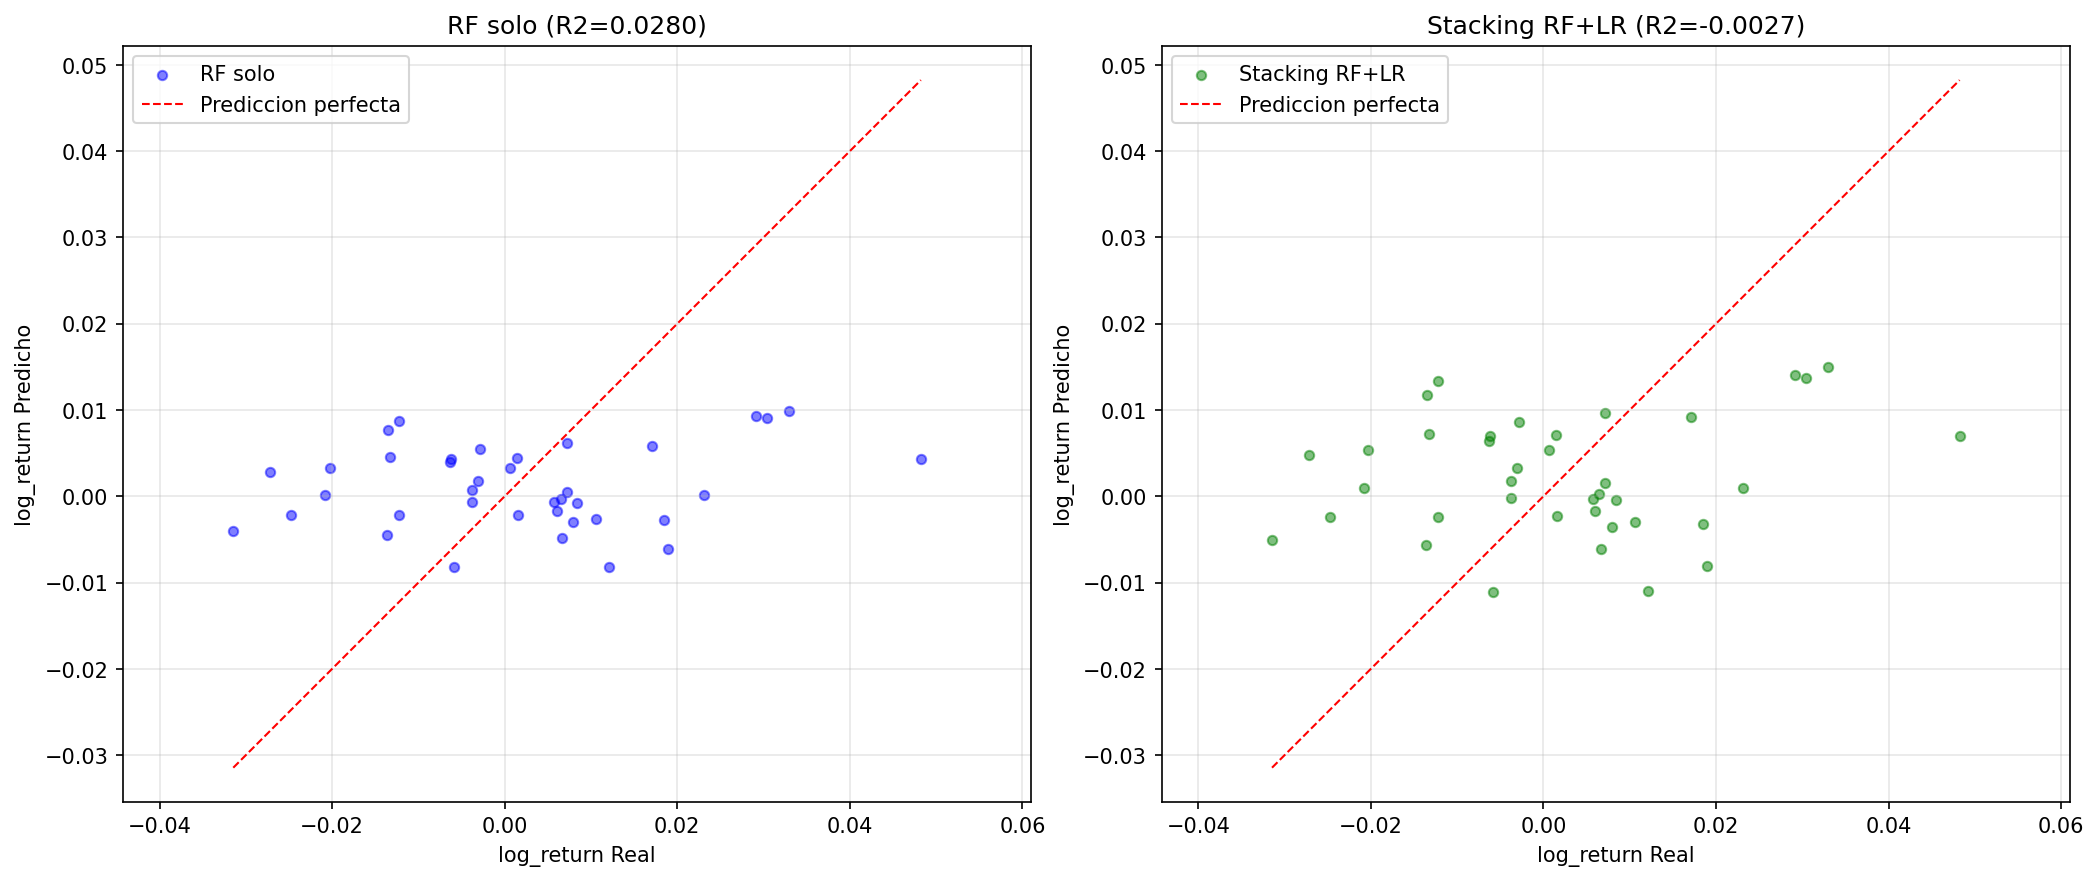
\includegraphics[width=0.75\textwidth]{../output/figures/models/predictions_log_return_v3.png}
    \caption{Retorno logar\'{\i}tmico real vs.\ predicho (RF v3) en el conjunto de prueba. Cada punto $( \hat{y}_i, y_i )$ representa un d\'{\i}a; la l\'{\i}nea diagonal $y=x$ indica predicci\'on perfecta.}
    \label{fig:scatter_logreturn}
\end{figure}

\subsubsection{Figura 2: Serie temporal del precio de cierre}

La Figura~\ref{fig:serie_close} presenta la evoluci\'on temporal del precio de cierre real de SBUX junto con las predicciones del modelo \textit{Random Forest} y del \textit{Stacking}, permitiendo visualizar el comportamiento del modelo a lo largo de los 38 d\'{\i}as del conjunto de prueba.

Para convertir las predicciones de retorno logar\'{\i}tmico $\hat{y}_i$ a precio de cierre predicho $\widehat{\text{Close}}_i$, se aplica la transformaci\'on inversa:
\[
\widehat{\text{Close}}_i = \text{Close}_{i-1} \cdot e^{\hat{y}_i}
\]
donde $\text{Close}_{i-1}$ es el precio de cierre real del d\'{\i}a anterior. Esta transformaci\'on es necesaria porque el modelo se entren\'o para predecir retornos (estacionarios) y no precios directamente.

\begin{figure}[H]
    \centering
    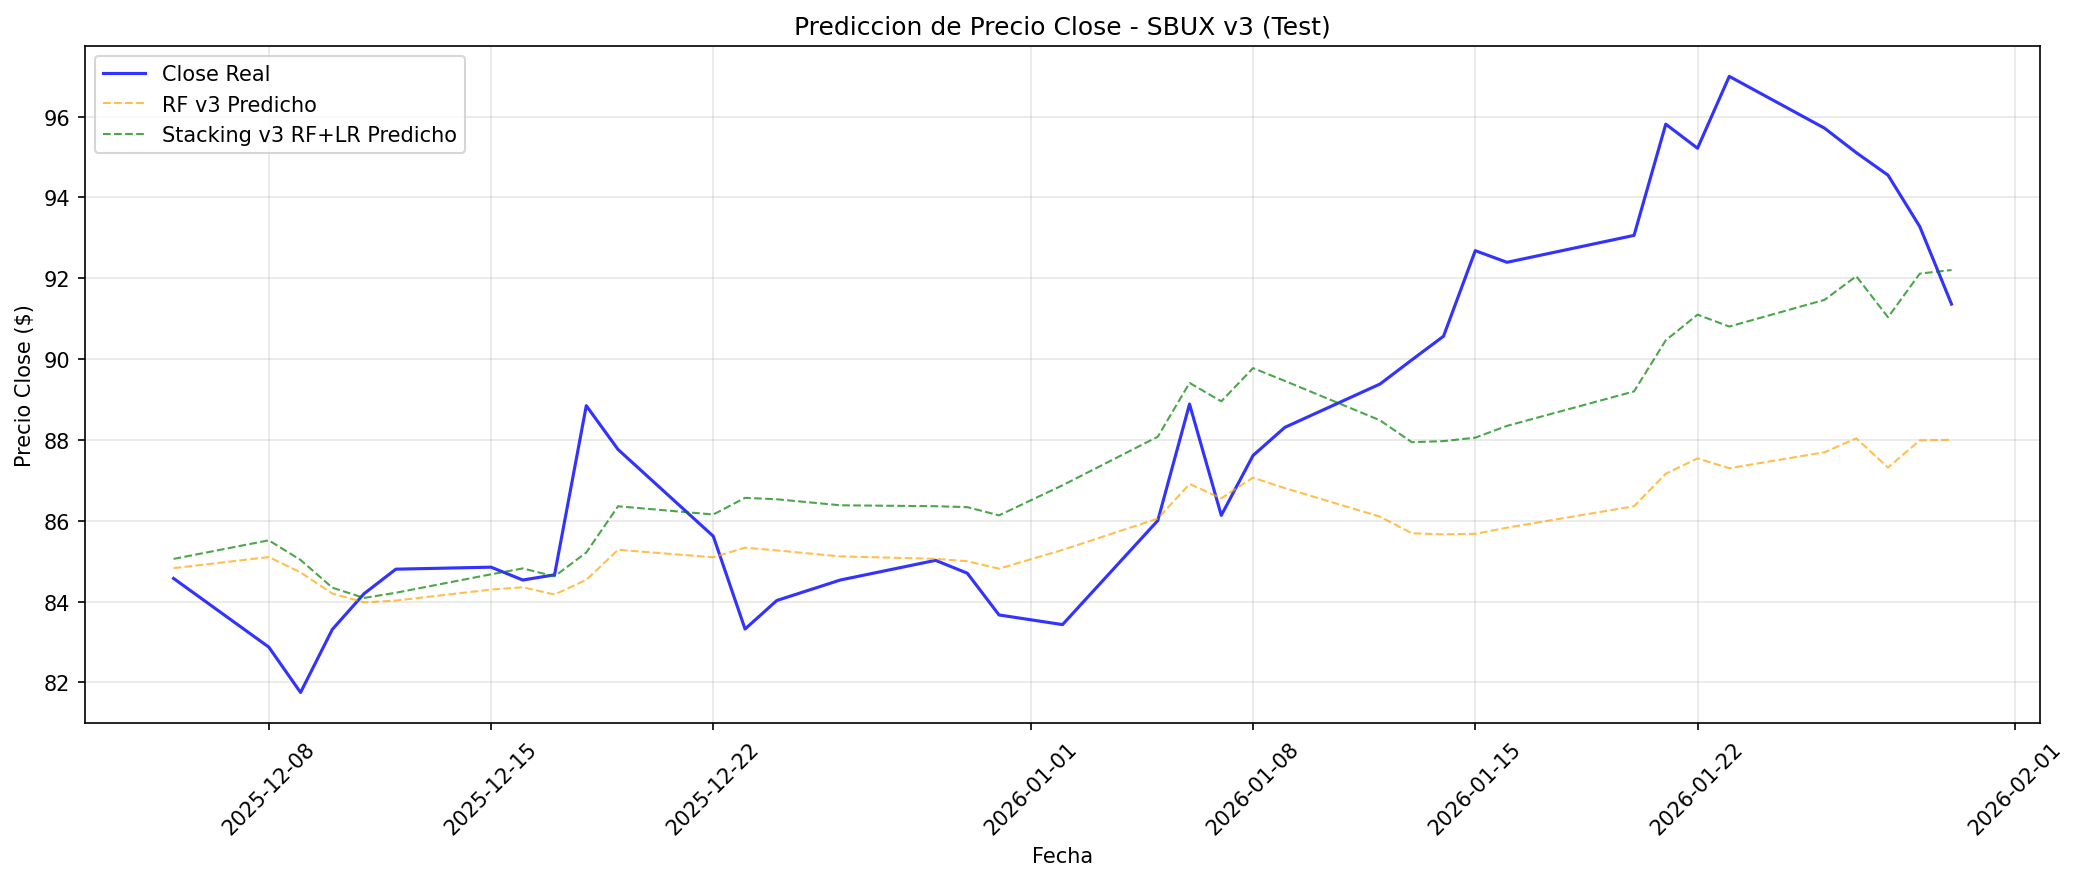
\includegraphics[width=0.75\textwidth]{../output/figures/models/predictions_close_v3.png}
    \caption{Serie temporal del precio de cierre real vs.\ predicciones de RF y Stacking en el conjunto de prueba.}
    \label{fig:serie_close}
\end{figure}

\subsubsection{Figura 3: Histograma de residuos}

La Figura~\ref{fig:histograma} muestra la distribuci\'on de los residuos $e_i = y_i - \hat{y}_i$ (diferencia entre el valor real y la predicci\'on), que es aproximadamente sim\'etrica y centrada en cero, indicando que el modelo no presenta sesgos sistem\'aticos marcados.

\begin{figure}[H]
    \centering
    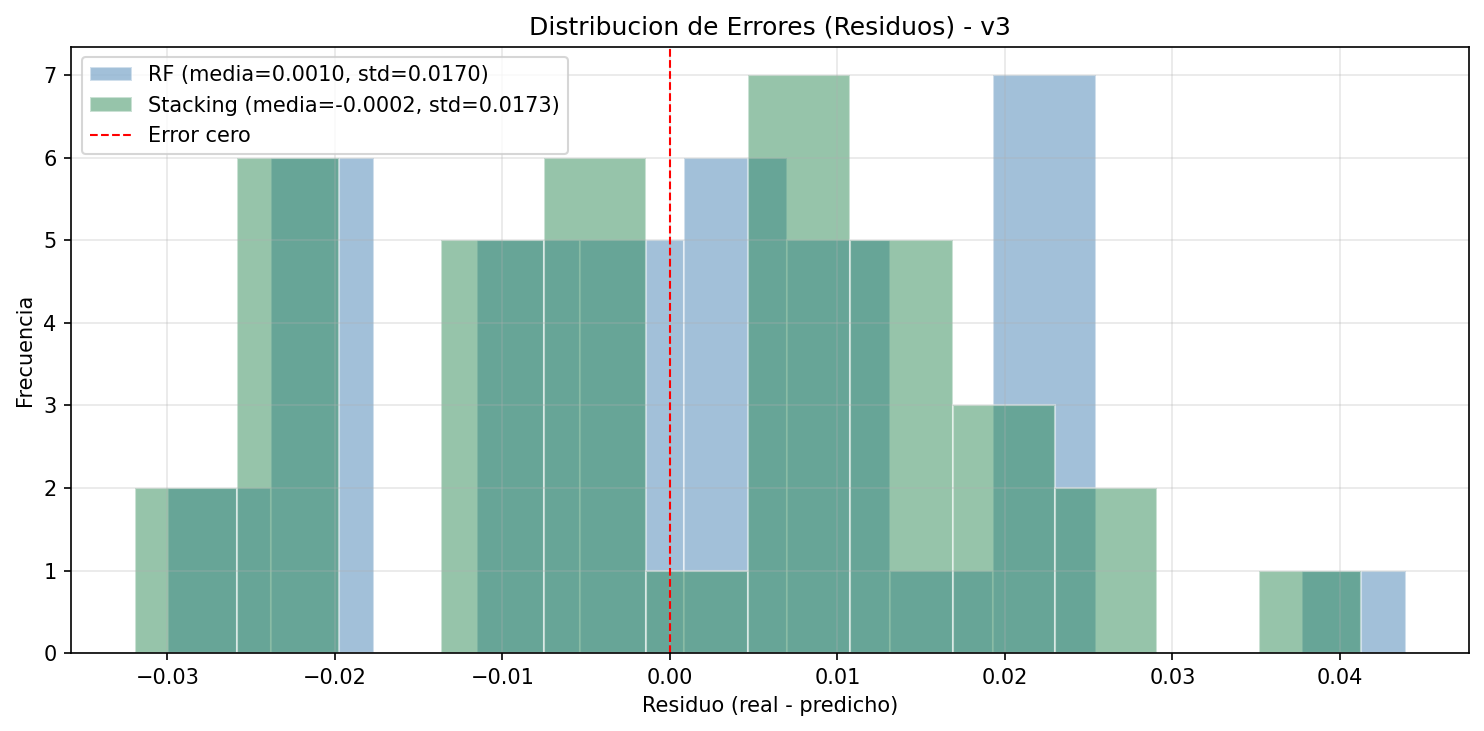
\includegraphics[width=0.75\textwidth]{../output/figures/models/predictions_error_histograma_v3.png}
    \caption{Histograma de los residuos del modelo RF v3. Una distribuci\'on sim\'etrica alrededor de cero indica ausencia de sesgo sistem\'atico.}
    \label{fig:histograma}
\end{figure}

\subsubsection{Figura 4: Dispersi\'on del precio de cierre}

La Figura~\ref{fig:scatter_close} presenta la relaci\'on entre el precio de cierre predicho y el real, ambos en unidades de d\'olares, lo que facilita la interpretaci\'on del desempe\~no del modelo en la escala original del problema.

Matem\'aticamente, esta figura es una transformaci\'on directa de la Figura~1. Dado el par de retornos $(\hat{y}_i, y_i)$ de la Figura~\ref{fig:scatter_logreturn}, se aplica la transformaci\'on exponencial a ambos ejes:
\[
\widehat{\text{Close}}_i = \text{Close}_{i-1} \cdot e^{\hat{y}_i}, \qquad
\text{Close}_i = \text{Close}_{i-1} \cdot e^{y_i}
\]
Cada punto $( \widehat{\text{Close}}_i, \text{Close}_i )$ se grafica en el plano. La l\'{\i}nea diagonal $y = x$ sigue representando la predicci\'on perfecta, pero ahora en la escala de precios original (d\'olares por acci\'on). La distancia vertical de cada punto a la diagonal es el error absoluto de predicci\'on en d\'olares.

\begin{figure}[H]
    \centering
    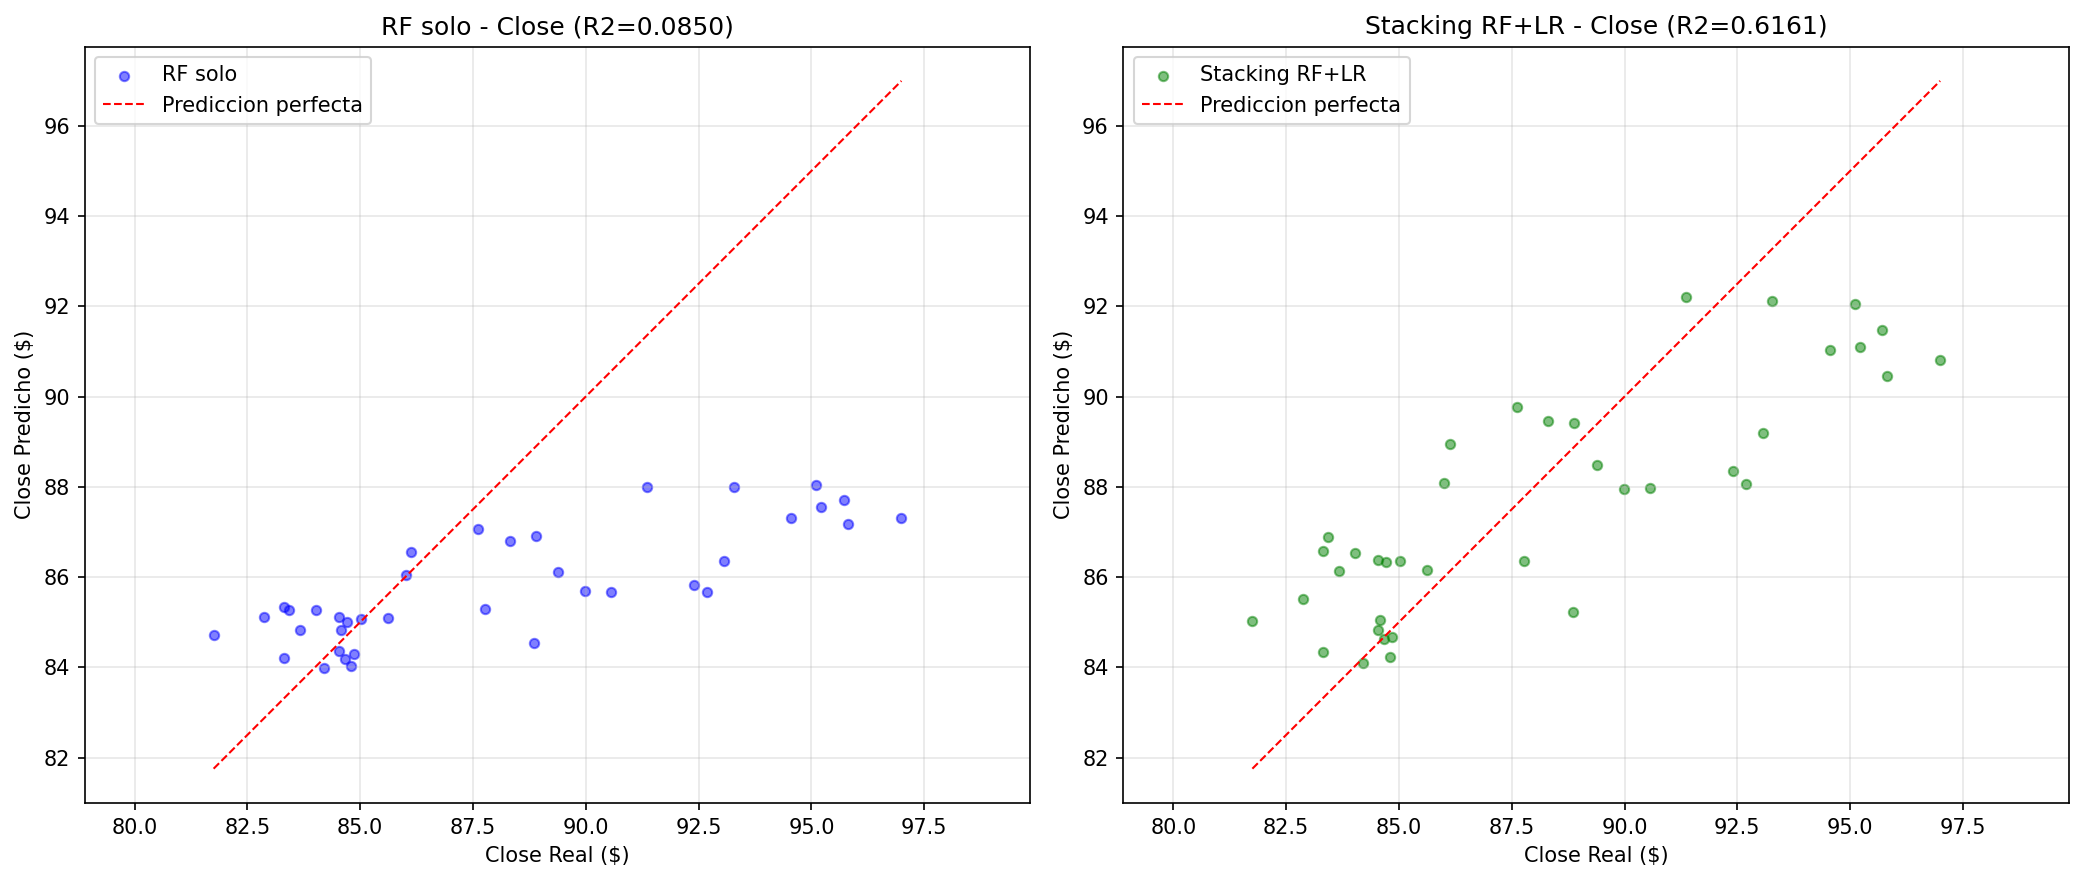
\includegraphics[width=0.75\textwidth]{../output/figures/models/predictions_close_scatter_v3.png}
    \caption{Precio de cierre predicho vs.\ real (RF v3) en unidades de d\'olares. Cada punto $( \widehat{\text{Close}}_i, \text{Close}_i )$ transforma el retorno logar\'{\i}tmico a precio original mediante $\widehat{\text{Close}}_i = \text{Close}_{i-1} \cdot e^{\hat{y}_i}$.}
    \label{fig:scatter_close}
\end{figure}

\subsection{Discusión}

El modelo \textit{Random Forest} versión~\textit{v3} logró un $R^{2}$ de 0.0280 en el conjunto de prueba, superando al modelo ingenuo de predecir la media ($R^{2}=0$) y a las versiones anteriores que utilizaban datos históricos desde 2015. Este resultado, aunque modesto, es consistente con la literatura de predicción de retornos financieros, donde valores de $R^{2}$ en el rango de 0.01 a 0.05 se consideran aceptables para modelos basados exclusivamente en datos históricos de precios \cite{gu2020empirical}.

El \textit{Stacking} con regresión lineal no mejoró al \textit{Random Forest} base en ninguna versión. Esto se atribuye a que la relación entre la predicción del RF y el valor real ya es aproximadamente lineal, por lo que la regresión lineal como meta-modelo introduce más sesgo del que logra corregir. En este contexto, el \textit{Random Forest} por sí solo ofrece el mejor equilibrio entre sesgo y varianza.

Las limitaciones principales de este trabajo son tres: (1) la señal predictiva en retornos financieros diarios es inherentemente débil, como postula la hipótesis de mercado eficiente; (2) el tamaño de la muestra de prueba (38 observaciones) limita la significancia estadística de las métricas; y (3) el modelo utiliza únicamente datos históricos de precio y volumen, sin incorporar variables macroeconómicas, indicadores de sentimiento de mercado ni noticias fundamentales de la empresa, que podrían aportar señal predictiva adicional.

\newpage

% ============================================================
% CONCLUSIÓN
% ============================================================
\section{Conclusión}
\label{sec:conclusion}

El presente trabajo tuvo como objetivo principal comprender el funcionamiento e interpretación de las métricas de evaluación en modelos de regresión, utilizando como caso de estudio la predicción del retorno logarítmico diario de las acciones de Starbucks (SBUX). Más que buscar un modelo financieramente operativo, se buscó desarrollar una comprensión práctica de cómo interpretar métricas como el MSE, RMSE, MAE, $R^{2}$, $R^{2}$ ajustado, correlación de Pearson, error máximo y sesgo, y entender por qué ciertas métricas ampliamente conocidas (como el MAPE) no son adecuadas para este tipo de problemas. El \textit{Random Forest} v3 demostró ser útil para este fin, alcanzando un $R^{2}$ de 0.028 y un RMSE de 0.0171, valores que, aunque modestos, permitieron ilustrar cada métrica en un contexto real.

Uno de los hallazgos metodológicos más importantes fue la necesidad de reducir la ventana de entrenamiento de diez años (2015--2024) a un solo año (2025--2026). Es importante destacar que este cambio no responde a una limitación en la cantidad de datos ---el algoritmo \textit{Random Forest} se beneficia de conjuntos grandes--- sino a la naturaleza de los mercados financieros, donde eventos externos impredecibles (cambios en la administración de la empresa, resultados trimestrales, políticas económicas, conflictos geopolíticos, entre otros) modifican radicalmente el régimen de mercado. Un modelo entrenado con datos de 2015 incluye períodos de expansión económica, la pandemia de COVID-19, picos inflacionarios y recuperaciones, todos ellos regímenes que no necesariamente se replican en el futuro inmediato. Al restringir el entrenamiento al último año, el modelo captura únicamente el régimen actual de SBUX, sacrificando cantidad de datos en favor de relevancia temporal.

Las cuatro gráficas presentadas en la sección de resultados se seleccionaron con propósitos complementarios. El gráfico de dispersión de retornos logarítmicos (Figura~\ref{fig:scatter_logreturn}) permite visualizar directamente la correlación entre predicción y valor real en la escala del \textit{target}, donde la distancia a la línea $y=x$ es el error de cada predicción; es la representación gráfica del $R^{2}$ y la correlación de Pearson. La serie temporal del precio de cierre (Figura~\ref{fig:serie_close}) transforma los retornos a la escala original en dólares, lo que permite evaluar si el modelo sigue la tendencia general del precio o si se desvía sistemáticamente en ciertos períodos; es particularmente útil para detectar sesgos temporales. El histograma de residuos (Figura~\ref{fig:histograma}) verifica uno de los supuestos fundamentales de los modelos de regresión: que los errores se distribuyan aproximadamente como una normal centrada en cero, lo cual es señal de un modelo bien especificado. Finalmente, el gráfico de dispersión del precio de cierre (Figura~\ref{fig:scatter_close}) lleva la evaluación al lenguaje del negocio (dólares por acción), facilitando la comunicación de los resultados a audiencias no técnicas.

Las limitaciones del estudio abren varias líneas de trabajo futuro. En primer lugar, la inclusión de variables fundamentales (estados financieros de SBUX, índices de referencia como el S\&P 500, tasas de interés) y de sentimiento de mercado (análisis de noticias, redes sociales) podría aumentar la señal predictiva más allá de los datos históricos de precio y volumen. En segundo lugar, la exploración de arquitecturas más complejas como LSTM (redes recurrentes) o \textit{Gradient Boosting} (XGBoost, LightGBM) podría capturar patrones no lineales que el \textit{Random Forest} no logra aprovechar. Por último, una reducción de características ---eliminando las variables temporales de baja importancia (\texttt{day\_of\_week} y \texttt{month} con menos del 3\% cada una)--- mejoraría el $R^{2}$ ajustado y la relación señal-ruido del modelo.

% ============================================================
% ANEXOS
% ============================================================
\newpage
\section{Anexos}
\label{sec:anexos}

\subsection{Anexo A: Tabla completa de métricas -- 3 versiones}

La Tabla~\ref{tab:anexo_metricas} presenta todas las métricas calculadas para las seis combinaciones de versión y modelo, incluyendo la correlación de Pearson (CC), el error máximo y el sesgo, que no se incluyeron en la tabla resumen de la Sección~\ref{sec:resultados} por claridad expositiva.

\begin{table}[H]
\centering
\caption{Comparación completa de métricas para las tres versiones exploradas.}
\label{tab:anexo_metricas}
\small
\begin{tabular}{lcccccccc}
\toprule
\textbf{Versión} & \textbf{Modelo} & \textbf{R$^{2}$} & \textbf{RMSE} & \textbf{MSE} & \textbf{MAE} & \textbf{CC} & \textbf{Max Err} & \textbf{Bias} \\
\midrule
v1 & RF & 0.0071 & 0.0211 & 0.000447 & 0.0146 & 0.1348 & 0.0624 & $-$0.0009 \\
v1 & Stacking RF+LR & $-$0.1460 & 0.0227 & 0.000516 & 0.0154 & 0.1348 & 0.0665 & $-$0.0009 \\
v2 & RF & $-$0.0102 & 0.0213 & 0.000455 & 0.0148 & 0.1102 & 0.0618 & $-$0.0008 \\
v2 & Stacking RF+LR & $-$0.1605 & 0.0229 & 0.000523 & 0.0155 & 0.1102 & 0.0652 & $-$0.0008 \\
\textbf{v3} & \textbf{RF} & \textbf{0.0280} & \textbf{0.0171} & \textbf{0.000291} & \textbf{0.0142} & \textbf{0.1941} & \textbf{0.0439} & \textbf{$-$0.0010} \\
v3 & Stacking RF+LR & $-$0.0027 & 0.0173 & 0.000301 & 0.0147 & 0.1941 & 0.0448 & $-$0.0011 \\
\bottomrule
\end{tabular}
\end{table}

\subsection{Anexo B: Código fuente de las funciones principales}

A continuación se describen las funciones principales implementadas en Python para el desarrollo de este trabajo. El código completo está disponible en el repositorio del proyecto.

\subsubsection{Ingeniería de características}

La función \texttt{build\_features()} toma el DataFrame con los datos OHLCV y construye las 10 características utilizadas por el modelo. Las transformaciones clave son:

\begin{itemize}
    \item \textbf{log\_return}: se calcula como \texttt{np.log(df['Close']).diff()}. Esta operación vectorizada genera el target estacionario y elimina la primera fila (NaN).
    \item \textbf{volatilidad\_20d y volatilidad\_5d}: se calculan con \texttt{df['log\_return'].rolling(window=N).std()}. La ventana desplazante (\textit{rolling window}) calcula la desviación estándar de los últimos $N$ retornos para cada día.
    \item \textbf{rango\_diario}: simplemente \texttt{df['High'] - df['Low']}. Esta característica captura la amplitud intradía sin introducir multicolinealidad.
    \item \textbf{log\_volume}: \texttt{np.log(df['Volume'])}. La transformación logarítmica comprime la cola larga de la distribución del volumen.
    \item \textbf{Lags}: \texttt{df['log\_return'].shift(k)} para $k \in \{1, 5, 20\}$. La función \texttt{shift()} desplaza la serie hacia adelante para crear rezagos temporales.
    \item \textbf{Dummies temporales}: \texttt{df['Date'].dt.dayofweek} y \texttt{df['Date'].dt.month}. El acceso \texttt{.dt} de pandas extrae componentes de fecha.
\end{itemize}

\subsubsection{División temporal y escalado}

A diferencia de la división aleatoria típica, aquí se respeta el orden cronológico:

\begin{itemize}
    \item Se ordenan los datos por fecha y se dividen secuencialmente: 70\% entrenamiento, 15\% validación, 15\% prueba.
    \item \texttt{StandardScaler} se ajusta (\texttt{fit}) exclusivamente con los datos de entrenamiento y luego se aplica (\texttt{transform}) a validación y prueba. Esto evita la fuga de información (\textit{data leakage}), ya que los parámetros de escala (media y desviación estándar) se derivan únicamente del conjunto de entrenamiento.
\end{itemize}

\subsubsection{Entrenamiento del Random Forest}

El modelo se entrena utilizando \texttt{RandomForestRegressor} de scikit-learn con búsqueda de hiperparámetros:

\begin{itemize}
    \item Se define una cuadrícula de hiperparámetros: \texttt{n\_estimators=100}, \texttt{max\_depth=10}, \texttt{min\_samples\_leaf=1}.
    \item El modelo se entrena con \texttt{model.fit(X\_train, y\_train)}.
    \item La evaluación en validación guía la selección de la mejor configuración.
    \item El modelo final se evalúa en el conjunto de prueba (no visto durante el entrenamiento ni la validación).
\end{itemize}

% ============================================================
% BIBLIOGRAFÍA
% ============================================================
\newpage
\bibliographystyle{plain}
\bibliography{../output/references}

% ============================================================
% (Las siguientes secciones se agregarán según confirmación)
% ============================================================

\end{document}
